% partes/parte1/cap01.tex
\chapter{El consumidor digital: evolución, impacto y ventajas de su análisis}
\label{cap:01}

\begin{cajaFicha}
\begin{description}
  \item[Unidad temática] I — Comportamiento, perfil y gestión de datos del consumidor digital.
  \item[Temas del programa] 1.1 Comportamiento del consumidor: 1.1.1 Evolución del consumidor 1.0 al 5.0 y tendencias a futuro; 1.1.2 Impacto del consumo digital inteligente y sostenible; 1.1.3 Ventajas del análisis del comportamiento del consumidor digital.
  \item[Horas] Teoría 2.0 · Práctica 4.0 · Aprendizaje autónomo 2.0.
  \item[Competencia de la unidad] Identifica el comportamiento del consumidor digital y su evolución a partir de sus tipos de perfil y gestión de datos.
  \item[Resultados de aprendizaje observables] Al concluir el capítulo, el estudiante:
  \begin{enumerate}
    \item distingue la evolución real del consumidor digital de su periodización comercial en \enquote{versiones};
    \item explica, con al menos dos fuentes verificables, qué significa consumo digital inteligente y sostenible en el contexto mexicano;
    \item argumenta, con datos, al menos tres ventajas concretas de analizar el comportamiento del consumidor digital para una organización.
  \end{enumerate}
  \item[Prerrequisitos] Ninguno formal; se recomienda familiaridad básica con conceptos de mercadotecnia general (mezcla de mercadotecnia, segmentación elemental).
\end{description}
\end{cajaFicha}

\section{Caso de apertura}

En 2015, el 57.4\,\% de la población mexicana de seis años o más usaba
internet. Diez años después, en 2025, esa cifra llegó a 86.1\,\%
\parencite{inegi2026endutih}. En el mismo periodo, el comercio electrónico
pasó de ser una curiosidad urbana a mover 941 mil millones de pesos anuales,
con 77.2 millones de compradores digitales \parencite{amvo2026}. Ninguna de
las dos cifras describe una revolución instantánea. Describen una curva:
lenta al principio, acelerada después, hoy cercana a su techo natural en
ciertos segmentos de la población y todavía lejos de él en otros (compárese
el 86.9\,\% de penetración urbana contra el 68.5\,\% rural en 2024;
\parencite{inegi2025endutih}). Este capítulo empieza ahí, con la pregunta que
suele saltarse en los diagnósticos de mercadotecnia: ¿la evolución del
consumidor digital es un fenómeno que se puede medir con esa curva, o es,
además, una narrativa que ciertas editoriales de consultoría han sabido
vender en entregas sucesivas? Las dos cosas son ciertas, y distinguirlas es
el primer ejercicio de rigor analítico que pide este libro.

\section{Desarrollo teórico}

\subsection{Evolución del consumidor: de la curva de adopción a la narrativa de versiones}
\progtag{1.1.1}

Dos relatos compiten para explicar cómo cambió el consumidor en las últimas
tres décadas. El primero es empírico: mide penetración de internet, uso de
dispositivos, volumen de transacciones digitales. El segundo es editorial:
organiza el cambio en versiones numeradas, del 1.0 al 6.0, cada una con un
librito que la anuncia. Conviene no confundirlos.

La serie \textit{Marketing X.0}, de Philip Kotler, Hermawan Kartajaya e Iwan
Setiawan, es el origen del segundo relato. \textit{Marketing 3.0} (2010)
proponía un giro hacia los valores del consumidor; \textit{Marketing 4.0}
(2016/2017), hacia la integración de lo digital y lo presencial;
\textit{Marketing 5.0} (2021), hacia la tecnología aplicada al factor humano
\parencite{kotler2021marketing50}; \textit{Marketing 6.0} (2024), hacia la
inmersión —internet de las cosas, inteligencia artificial, realidad
aumentada— bajo la etiqueta de \enquote{metamarketing} \parencite{kotler2024marketing6}.
La figura~\ref{fig:cap01-lineamx0} muestra esta secuencia.

\begin{figure}[htbp]
  \centering
  % figuras/tikz/cap01-linea-marketing-x0.tex
% Línea de tiempo crítica: la serie "Marketing X.0" de Kotler, Kartajaya y Setiawan
% como periodización editorial (no modelo académico validado empíricamente).
\begin{tikzpicture}[
    hito/.style={rectangle, rounded corners, draw=guindaIPN, thick, fill=guindaIPNClara,
                 minimum width=2.6cm, minimum height=1.4cm, align=center, font=\footnotesize},
    linea/.style={thick, draw=grisIPN}
  ]
  \draw[linea, -{Stealth[length=3mm]}] (-0.3,0) -- (13.3,0);

  \node[hito] (m1) at (0,0.9) {\textbf{1.0}\\[1pt] Producto\\ (s.\,f.)};
  \node[hito] (m2) at (3.3,0.9) {\textbf{2.0}\\[1pt] Consumidor\\ (s.\,f.)};
  \node[hito] (m3) at (6.6,0.9) {\textbf{3.0}\\[1pt] Valores\\ 2010};
  \node[hito] (m4) at (9.9,0.9) {\textbf{4.0}\\[1pt] Digital\\ 2016};
  \node[hito] (m5) at (13.2,0.9) {\textbf{5.0}\\[1pt] Tecnología\\ 2021};

  \foreach \x in {0,3.3,6.6,9.9,13.2} {
    \draw[linea] (\x,0) -- (\x,0.2);
  }

  \node[hito, fill=bronceIPNClaro, draw=bronceIPN] (m6) at (13.2,-1.3) {\textbf{6.0}\\[1pt] Inmersivo\\ 2024};
  \draw[linea] (13.2,-0.2) -- (13.2,-0.6);

  \node[align=center, font=\scriptsize\itshape, text width=13.5cm] at (6.5,-2.6)
    {Serie editorial de libros (Kotler, Kartajaya y Setiawan), no un programa de\\
     investigación arbitrado: cada entrega se alinea a la tecnología dominante de su año de publicación.};
\end{tikzpicture}

  \caption{La serie \enquote{Marketing X.0} como periodización editorial. Cada
  entrega se publica alineada a la tecnología dominante de su momento; no es
  un programa de investigación con aparato empírico propio ni revisión por
  pares. Fuente: elaboración propia con base en
  \parencite{kotler2021marketing50,kotler2024marketing6}.}
  \label{fig:cap01-lineamx0}
\end{figure}

Cada entrega de la serie es útil como lectura de tendencias de la práctica
profesional. Ninguna es, en el sentido estricto, un modelo académico
validado: no hay una teoría del consumidor 4.0 sometida a revisión por pares
con la misma exigencia metodológica que, por ejemplo, la teoría de la
segmentación de mercado de Wendell Smith, publicada casi setenta años antes
en el \textit{Journal of Marketing} \parencite{smith1956}. Esta distinción no
resta valor a la serie de Kotler et al. como diagnóstico de industria. Sí
exige presentarla con el estatus que le corresponde: una lectura influyente
de consultoría, no un hecho histórico objetivo. El libro más reciente sobre
comportamiento del consumidor digital que localizamos, de Jagdish Sheth y
Varsha Jain \parencite{sheth2026}, evita la lógica de versiones y organiza el
cambio por mecanismos —qué datos genera el consumidor, cómo se procesan, qué
decisiones habilitan— en vez de por eras. Es un contraste metodológico que
vale la pena señalar al estudiante: hay más de una forma legítima de narrar
el mismo cambio.

¿Qué cambió entonces, de forma verificable? Tres cosas, con evidencia
directa: la proporción de la población con acceso a internet (evidencia en
\S\ref{sec:cap01-evidencia}), el tipo de decisiones que se toman en entornos
digitales en vez de presenciales, y la cantidad de rastro de datos que cada
decisión deja disponible para el análisis. Este último punto es el que abre
el resto del libro: no es solo que el consumidor cambió, es que ahora se
puede observar de una manera que antes no existía.

Esa posibilidad de observación introduce la tensión de fondo que recorre
todo el libro: el consumidor digital tiene una doble naturaleza, es persona
vivida y es, simultáneamente, dato estructurado disponible para el análisis
(figura~\ref{fig:cap01-doble-naturaleza}). Ninguna de las dos lecturas basta
por sí sola —una organización que solo ve datos pierde el contexto humano de
la decisión; una que solo ve personas no puede operar a la escala que exige
un mercado digital de millones de usuarios—, y sostener las dos en tensión,
sin colapsar en ninguna, es la competencia central que este libro busca
desarrollar.

\begin{figure}[htbp]
  \centering
  % figuras/tikz/cap01-doble-naturaleza.tex
% Diagrama conceptual: el consumidor digital como persona vivida y como dato
% estructurado — las dos lecturas que el capítulo pide distinguir.
\begin{tikzpicture}[
    caja/.style={rectangle, rounded corners, draw=guindaIPN, thick, fill=guindaIPNClara,
                 minimum width=5cm, minimum height=2.6cm, align=center, font=\small},
    etiqueta/.style={font=\scriptsize\itshape, text width=5cm, align=center},
    flecha/.style={-{Stealth[length=2.5mm]}, thick, draw=doradoIPN}
  ]
  \node[caja] (persona) at (0,0) {\textbf{Consumidor}\\ como persona\\[4pt]
    necesidad, deseo,\\ contexto, emoción};
  \node[caja] (dato) at (7,0) {\textbf{Consumidor}\\ como dato\\[4pt]
    clic, sesión, patrón,\\ variable de un modelo};

  \draw[flecha] (persona) -- node[above, font=\scriptsize, align=center] {se registra\\ como} (dato);
  \draw[flecha] (dato) to[bend left=25] node[below, font=\scriptsize] {predice y moldea} (persona);

  \node[etiqueta] at (0,-1.9) {Unidad de análisis: la experiencia individual};
  \node[etiqueta] at (7,-1.9) {Unidad de análisis: el agregado estadístico};
\end{tikzpicture}

  \caption{El consumidor digital como persona vivida y como dato
  estructurado: dos unidades de análisis en tensión permanente. Fuente:
  elaboración propia.}
  \label{fig:cap01-doble-naturaleza}
\end{figure}

\subsection{Impacto del consumo digital inteligente y sostenible}
\progtag{1.1.2}

\enquote{Consumo inteligente} y \enquote{consumo sostenible} no son sinónimos, aunque el
discurso de mercadotecnia digital tiende a fusionarlos. El primero se refiere
a decisiones de compra informadas por datos y comparación (uso de
comparadores de precio, lectura de reseñas, verificación de especificaciones
técnicas antes de comprar). El segundo se refiere al impacto ambiental y
social de esas decisiones, con independencia de qué tan informadas estén.

En México, PROFECO ha incorporado explícitamente el lenguaje de la economía
circular en su comunicación al consumidor: la Revista del Consumidor dedicó
en septiembre de 2025 un número a la vida útil de los dispositivos
electrónicos y a la compra de productos remanufacturados, con el objetivo
declarado de evitar el \textit{greenwashing} —reclamos ambientales que no se
pueden verificar— mediante etiquetado responsable
\parencite{profeco2025entornodigital}. El marco internacional de referencia
es el Objetivo de Desarrollo Sostenible 12 de la ONU, Producción y Consumo
Responsables \parencite{onu2015ods12}, que sitúa el consumo digital dentro de
un problema más amplio: la producción de dispositivos, servidores y
conectividad tiene un costo ambiental que la conversación de mercadotecnia
digital, centrada casi siempre en la conversión y la retención, tiende a dejar
fuera del análisis.

\begin{cajaFrontera}
\textbf{Consumo sostenible: la brecha entre actitud y conducta.}
Que un consumidor declare preferencia por productos sostenibles no significa
que los compre. La literatura académica llama a esto \textit{brecha
actitud-conducta} (\textit{attitude-behavior gap}): la actitud pro-ambiental
autoinformada predice, de forma sistemática, peor la conducta de compra real
de lo que predeciría un modelo de conducta planeada bien especificado —entran
en juego el precio relativo, la conveniencia percibida y la confianza en que
la etiqueta ambiental sea cierta. No localizamos, al cierre de esta
investigación, un estudio con cifras específicas de esta brecha para el
mercado mexicano: es una oportunidad de indagación documental legítima para
el portafolio de evidencias de este capítulo, no un hueco que debamos llenar
con una cifra sin verificar.
\end{cajaFrontera}

\subsection{Ventajas del análisis del comportamiento del consumidor digital}
\progtag{1.1.3}

¿Para qué le sirve a una organización analizar sistemáticamente el
comportamiento de su consumidor digital, más allá de la intuición del
equipo de mercadotecnia? El cuadro~\ref{tab:cap01-ventajas} resume cuatro
ventajas con distinto nivel de evidencia, deliberadamente clasificadas para
que el estudiante distinga la que está bien establecida en la literatura de
la que es, todavía, promesa de proveedor de tecnología.

\begin{table}[htbp]
\centering
\begin{tabular}{@{}p{3.2cm}p{6.3cm}p{3.5cm}@{}}
\toprule
Ventaja & Descripción & Nivel de evidencia \\
\midrule
Segmentación más precisa & Agrupar consumidores por comportamiento observado, no solo por variables demográficas declaradas & Alto — literatura arbitrada desde Smith (1956) \\
Personalización de la oferta & Ajustar producto, precio o mensaje al perfil inferido del consumidor & Medio — efectividad documentada, pero con límites (fatiga de personalización, percepción de vigilancia) \\
Reducción de fricción en el recorrido & Detectar en qué punto del proceso de decisión abandona el consumidor y corregirlo & Alto — instrumentable directamente con analítica de embudo \\
Anticipación de tendencias & Detectar cambios de comportamiento antes que la competencia & Bajo-medio — depende de la calidad y representatividad del dato, riesgo de sobreajuste a ruido \\
\bottomrule
\end{tabular}
\caption{Ventajas del análisis del comportamiento del consumidor digital,
clasificadas por nivel de evidencia. Fuente: elaboración propia con base en
\parencite{smith1956,solomon2017,sheth2026}.}
\label{tab:cap01-ventajas}
\end{table}

La cuarta fila merece una advertencia explícita. \enquote{Anticipar tendencias} es la
promesa más común del discurso comercial de analítica de consumidor y la
menos sostenida por evidencia sistemática: un patrón detectado en datos
históricos no garantiza que se repita, y la literatura de economía
conductual documenta cómo los propios analistas caen en el sesgo de
representatividad al proyectar continuidad donde solo hubo una coincidencia
\parencite{tverskykahneman1974}. Este es el primer contacto del libro con un
tema que reaparecerá en los capítulos 5 y 10--11: los datos no eliminan el
sesgo humano en la toma de decisiones, lo pueden amplificar si no se
interpretan con criterio.

\section{Evidencia de México y del mundo}
\label{sec:cap01-evidencia}

\begin{table}[htbp]
\centering
\begin{tabular}{@{}lrr@{}}
\toprule
Indicador & 2024 & 2025 \\
\midrule
Población de 6+ años que usa internet & 83.1\,\% & 86.1\,\% \\
Adopción de internet, zona urbana & 86.9\,\% & — \\
Adopción de internet, zona rural & 68.5\,\% & — \\
Compradores digitales en México & — & 77.2 millones \\
Valor del comercio electrónico (crecimiento anual) & — & \$941{,}000 mdp (+19.2\,\%) \\
\bottomrule
\end{tabular}
\caption{Evolución reciente del consumidor digital en México. Fuente:
elaboración propia con datos de INEGI, ENDUTIH 2024 y 2025
\parencite{inegi2025endutih,inegi2026endutih}, y AMVO, Estudio de Venta
Online 2026 \parencite{amvo2026}.}
\label{tab:cap01-evidencia}
\end{table}

Dos lecturas se desprenden del cuadro~\ref{tab:cap01-evidencia}. La primera:
el crecimiento de la conectividad en México no se ha detenido, pero tampoco
es parejo —la brecha urbano-rural de dieciocho puntos porcentuales en 2024 es
más relevante para la práctica profesional que la cifra nacional agregada,
porque delimita en qué proporción del país una estrategia \enquote{todo digital} es
viable sin canales complementarios. La segunda: el crecimiento del comercio
electrónico (+19.2\,\% anual) supera al crecimiento de la conectividad
misma, lo que sugiere que buena parte del aumento no viene de gente nueva
conectándose, sino de gente ya conectada que compra más. Es una distinción
que el capítulo 3 retoma al hablar de toma de decisiones basadas en gestión
de datos.

\begin{cajaEtica}
Toda cifra de este capítulo proviene de fuente primaria verificable (INEGI,
AMVO) o está explícitamente marcada como estimación provisional. Ninguna
cifra de crecimiento o de tamaño de mercado citada en este libro se presenta
sin su fuente, año y fecha de consulta. Esto no es solo una norma editorial:
es el mismo estándar que el capítulo pide exigirle a cualquier proveedor de
analítica de consumidor que presente una cifra sin metodología pública.
Desconfiar de un dato no verificable es, en sí mismo, una competencia
profesional de mercadotecnia digital.
\end{cajaEtica}

\section{Laboratorio MATLAB: difusión de la adopción de un canal digital}

\begin{cajaLaboratorio}
\textbf{Objetivo.} Simular, con el modelo de Bass, cómo la proporción entre
adopción por innovación (decisión independiente) y adopción por imitación
(contagio social) cambia la forma de la curva de adopción de un canal
digital, e interpretar esa forma en términos de estrategia de lanzamiento.

\textbf{Concepto detrás del código.} El modelo de Bass \parencite{bass1969}
describe la tasa de adopción de una innovación como
\[
  \frac{dF(t)}{dt} = \big(p + q\,F(t)\big)\big(1 - F(t)\big),
\]
donde $F(t)$ es la fracción acumulada del mercado potencial que ya adoptó al
tiempo $t$, $p$ es el coeficiente de innovación y $q$ el de imitación. La
solución cerrada de esta ecuación diferencial,
\[
  F(t) = \frac{1 - e^{-(p+q)t}}{1 + \tfrac{q}{p}\,e^{-(p+q)t}},
\]
es la que implementa el script. El punto de inflexión de la curva —el
momento de máxima velocidad de adopción— ocurre en
$t^\ast = \ln(q/p)\,/\,(p+q)$: cuanto mayor es $q$ respecto a $p$, más tarde y
más abrupto es ese pico, porque la adopción depende más del contagio social
que de decisiones independientes.

\textbf{Script.} \texttt{matlab/cap01/cap01\_difusion\_bass.m}. Es el
\textbf{mismo script, sin modificar}, que se usa en la Práctica 1 de esta
Parte: toda la lógica de cálculo y graficación está fija; lo único que el
estudiante edita es el bloque de \textbf{parámetros}, claramente delimitado
al inicio del archivo. Corrida tal como está, usa parámetros
\textbf{didácticos} ($p=0.03$, $q=0.38$), no calibrados con datos reales de
un canal digital mexicano —decisión editorial deliberada, para mantener el
ejercicio enfocado en la forma de la curva y no en la calibración
estadística.

\begin{lstlisting}[style=MATLABStyle, caption={Bloque de parámetros editable (\texttt{cap01\_difusion\_bass.m}) — es lo único que cambia entre corridas.}]
p = 0.03;      % coeficiente de innovacion
q = 0.38;      % coeficiente de imitacion
m = 1;         % mercado potencial (normalizado)
tFinal = 20;   % periodos a simular
\end{lstlisting}

\textbf{Salida esperada.} Al correr el script (\texttt{Run}, sin editar nada
más que el bloque de parámetros) se imprimen en la ventana de comandos el
periodo del pico de adopción y el porcentaje de mercado adoptado al final del
periodo simulado, y se generan dos figuras: adopción acumulada
(figura~\ref{fig:cap01-bass-acum}) y tasa de adopción
(figura~\ref{fig:cap01-bass-tasa}), ambas con los valores de $p$ y $q$
usados en el título, para poder identificar de qué corrida viene cada una.

\begin{center}
  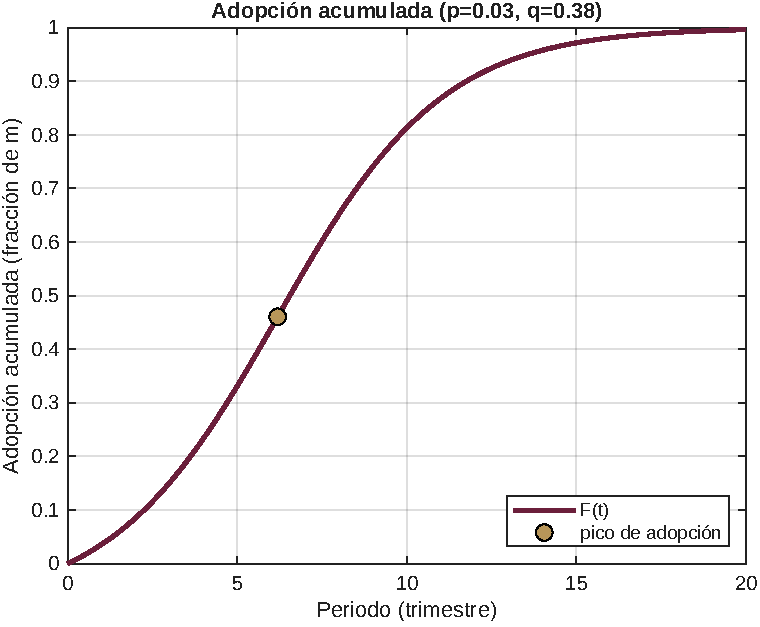
\includegraphics[width=0.75\textwidth]{figuras/matlab/cap01_bass_acumulada.pdf}
  \captionof{figure}{Adopción acumulada del modelo de Bass, parámetros
  didácticos ($p=0.03$, $q=0.38$). Fuente: elaboración propia con datos
  sintéticos, \texttt{rng(42)}.}
  \label{fig:cap01-bass-acum}
\end{center}

\begin{center}
  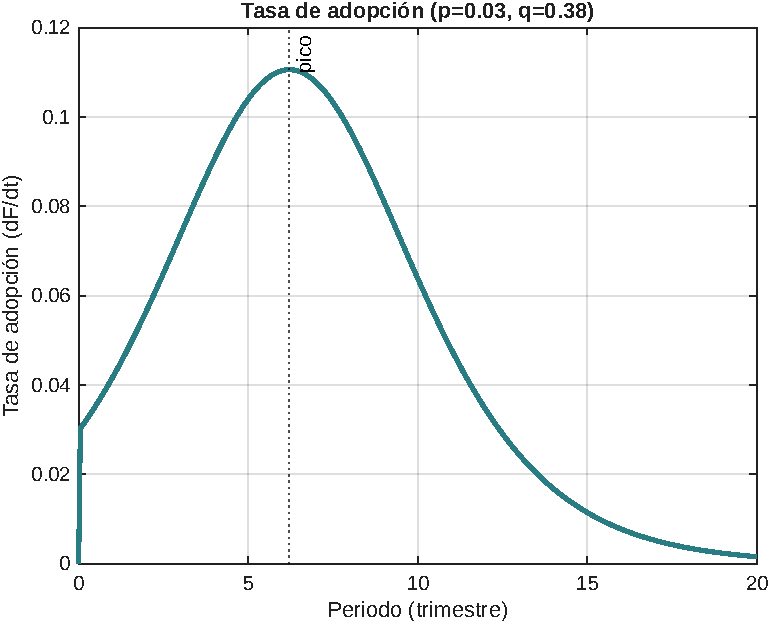
\includegraphics[width=0.75\textwidth]{figuras/matlab/cap01_bass_tasa.pdf}
  \captionof{figure}{Tasa de adopción del modelo de Bass, misma corrida.
  Fuente: elaboración propia con datos sintéticos.}
  \label{fig:cap01-bass-tasa}
\end{center}

\textbf{Interpretación de negocio.} El pico de esta corrida ($p=0.03$,
$q=0.38$) ocurre en $t^\ast \approx 6.2$ periodos, con 46\,\% del mercado ya
adoptado en ese momento. Cuanto mayor es $q$ respecto a $p$, más tarde y más
abrupto es ese pico —porque la adopción depende más del contagio social que
de decisiones independientes—, lo que en la figura se traduce en una fase
inicial más plana seguida de un despegue más pronunciado. El ejercicio
propuesto pide comprobar esto de primera mano, no como afirmación del libro.

\textbf{Ejercicio propuesto (usen exactamente este script, solo cambien el
bloque de parámetros).} Corran el script tres veces, una por caso, y
completen un cuadro con los resultados que imprime cada corrida:
\begin{enumerate}
  \item \textbf{Caso A — innovación dominante:} $p=0.08$, $q=0.10$.
  \item \textbf{Caso B — balance:} $p=0.03$, $q=0.38$ (los valores por defecto del script).
  \item \textbf{Caso C — imitación dominante:} $p=0.01$, $q=0.55$.
\end{enumerate}
Para cada caso, registren: el periodo del pico ($t^\ast$), el porcentaje de
mercado adoptado en ese pico, y el porcentaje de mercado adoptado al periodo
20. Con el cuadro completo, respondan por escrito: ¿en qué caso el pico
ocurre más tarde? ¿En qué caso la curva de adopción acumulada tiene una fase
inicial más plana? A partir de sus tres corridas —no de este libro—,
propongan un canal digital real (una app, una red social, un método de
pago) y justifiquen a cuál de los tres casos se parece más su patrón de
adopción esperado.

\textbf{Extensión opcional.} Investigar el modelo de Bass generalizado (con
coeficiente de presión de precio o de publicidad variable en el tiempo) y
describir, sin necesariamente programarlo, qué cambiaría en la forma de la
curva de este script.
\end{cajaLaboratorio}

\section{Estudio de caso}

\begin{casoFicticio}
Una fintech mexicana lanza una app de ahorro programado dirigida a
trabajadores independientes. A los tres meses del lanzamiento, la app tiene
2{,}000 usuarios activos —muy por debajo de la proyección inicial de 15{,}000—
y el equipo directivo discute si el producto \enquote{no funciona} o si simplemente
necesita más tiempo. El equipo de datos presenta dos lecturas alternativas de
la misma curva de adopción observada: una consistente con un canal dominado
por innovación (crecimiento lento pero sostenido, sin señales de contagio
entre usuarios), y otra consistente con un canal dominado por imitación
(la app apenas está saliendo del \enquote{valle} inicial y podría acelerar pronto si
el referido entre usuarios empieza a operar).

\textbf{Preguntas guía.}
\begin{enumerate}
  \item ¿Qué evidencia adicional —más allá del conteo de usuarios activos— permitiría distinguir entre las dos lecturas del caso?
  \item Si el diagnóstico correcto fuera \enquote{canal dominado por imitación en fase de valle}, ¿qué decisión de mercadotecnia sería la más riesgosa tomar en este momento?
  \item ¿Qué papel jugaría un programa de referidos en cambiar el balance entre $p$ y $q$ de este producto?
  \item Relacione este caso con la distinción entre \enquote{narrativa de versiones} y \enquote{evolución verificable} del \S 2.1: ¿qué tipo de evidencia usaría el equipo directivo para justificar su decisión frente a la dirección general, y por qué esa evidencia debe ser de fuente primaria?
\end{enumerate}
\end{casoFicticio}

\section{Actividades y evidencias del portafolio}

Alineadas con la estrategia oficial de la unidad (estudio de casos) y el
portafolio de evidencias de la Unidad I:

\begin{description}
  \item[Reporte de indagación documental] En equipos de tres a cuatro
  integrantes, investigar y contrastar dos fuentes académicas o
  institucionales (no blogs) sobre un concepto del capítulo no desarrollado
  en profundidad en el texto (p.\ ej., el marco de los cuatro niveles de la
  brecha digital, o el estado más reciente del comercio electrónico
  fronterizo). Criterio de evaluación: cada afirmación con cifra debe llevar
  fuente, año y fecha de consulta.
  \item[Exposición] Presentar en 8 minutos la comparación entre la
  \enquote{narrativa de versiones} (Marketing X.0) y la evolución verificable del
  consumidor digital mexicano, con al menos un dato de INEGI o AMVO no citado
  en este capítulo. Criterio de evaluación: distinción clara entre fuente
  primaria y lectura de consultoría.
  \item[Solución de casos] Resolver el estudio de caso de la fintech
  (\S 2.5) por escrito, con las cuatro preguntas guía respondidas y una
  recomendación final justificada.
  \item[Reporte de debate] En sesión plenaria, debatir la pregunta: \enquote{¿El
  consumo digital inteligente y el consumo sostenible son objetivos
  compatibles o están en tensión?}, con al menos una postura respaldada en la
  brecha actitud-conducta (recuadro de Frontera, \S 2.2).
  \item[Reporte de práctica] Entregar el cuadro de los tres casos del
  ejercicio propuesto del laboratorio (\S 3) —sin modificar el script, solo
  el bloque de parámetros— con las dos preguntas de comparación respondidas
  y la propuesta de canal digital real justificada.
\end{description}

\section{Ruta de aprendizaje autónomo}

Dos horas de aprendizaje autónomo asignadas a este capítulo. Tareas
concretas:
\begin{enumerate}
  \item Leer el comunicado de prensa más reciente de ENDUTIH (INEGI) y
  extraer tres cifras no citadas en este capítulo, con su fuente exacta.
  \item Revisar la ficha editorial de \textit{Marketing 6.0}
  \parencite{kotler2024marketing6} y anotar, en dos párrafos, si las
  tendencias que anuncia (inmersión, IA, IoT) ya son observables en algún
  servicio digital que el estudiante use cotidianamente.
  \item Ejecutar el script \texttt{cap01\_difusion\_bass.m} con los
  parámetros propios del ejercicio propuesto (\S 3) y anotar el tiempo del
  pico de adopción resultante.
\end{enumerate}

\section{Síntesis}

La evolución del consumidor digital admite dos lecturas que no deben
confundirse: una curva medible de adopción de tecnología y una narrativa
editorial organizada en versiones. Ambas son útiles; solo una es evidencia.
El consumo digital inteligente (decisiones informadas por datos) y el consumo
sostenible (decisiones con menor costo ambiental) son fenómenos distintos que
el discurso de mercadotecnia tiende a fusionar sin evidencia suficiente de
que coincidan en la práctica —la brecha actitud-conducta documenta
precisamente esa distancia. Analizar el comportamiento del consumidor digital
trae ventajas con niveles de evidencia desiguales: la segmentación basada en
comportamiento observado y la reducción de fricción en el recorrido de compra
están bien sustentadas; la anticipación de tendencias, la menos.

\subsection*{Glosario del capítulo}
\begin{description}
  \item[Brecha actitud-conducta] Distancia entre lo que un consumidor declara
  preferir y lo que efectivamente compra.
  \item[Consumo digital inteligente] Decisiones de compra informadas por
  datos y comparación en entornos digitales.
  \item[Coeficiente de imitación ($q$)] En el modelo de Bass, parámetro que
  mide cuánto depende la adopción del contagio social entre adoptantes.
  Rango matemático válido: $q \geq 0$ (sin cota superior estricta); en los
  casos didácticos de este libro se usan valores entre 0.10 y 0.55.
  \item[Coeficiente de innovación ($p$)] En el modelo de Bass, parámetro que
  mide la propensión a adoptar de forma independiente, sin influencia social.
  Rango matemático válido: $p > 0$ (si $p=0$, nadie inicia la adopción); en
  los casos didácticos de este libro se usan valores entre 0.01 y 0.08.
  \item[Mercado potencial ($m$)] En el modelo de Bass, tamaño del mercado
  objetivo, normalizado a 1 en este libro (equivale al 100\,\% del mercado).
  Rango: $m > 0$; con $m=1$, la adopción acumulada $F(t)$ queda expresada
  directamente como fracción del mercado.
  \item[\textit{Greenwashing}] Comunicación de atributos ambientales de un
  producto que no se pueden verificar o que exageran su impacto real.
\end{description}

\subsection*{Autoevaluación}

\textbf{Opción múltiple}

\begin{enumerate}
  \item La serie de libros \textit{Marketing X.0} (Kotler, Kartajaya y
  Setiawan) debe entenderse principalmente como:
  \begin{enumerate}
    \item[a)] Un programa de investigación académica revisado por pares.
    \item[b)] Una periodización editorial de consultoría alineada a la tecnología de cada momento. \textit{(correcta)}
    \item[c)] El primer marco teórico sobre comportamiento del consumidor digital.
    \item[d)] Una norma internacional de mercadotecnia digital.
  \end{enumerate}
  \textit{Justificación:} el capítulo documenta que cada entrega se publica
  alineada a la tecnología dominante de su año, sin aparato empírico propio
  ni revisión por pares (\S 2.1).

  \item En el modelo de Bass, si $q \gg p$, la curva de adopción se
  caracteriza por:
  \begin{enumerate}
    \item[a)] Crecimiento lineal y constante desde el inicio.
    \item[b)] Una fase inicial plana seguida de adopción explosiva. \textit{(correcta)}
    \item[c)] Adopción inmediata de todo el mercado potencial.
    \item[d)] Ausencia total de adopción.
  \end{enumerate}
  \textit{Justificación:} cuando la imitación domina, la adopción depende del
  contagio social, que requiere una base inicial de adoptantes antes de
  acelerar — comprobado en el ejercicio propuesto del \S 3 (Caso C).

  \item La brecha actitud-conducta en consumo sostenible se refiere a:
  \begin{enumerate}
    \item[a)] La diferencia de precio entre productos sostenibles y convencionales.
    \item[b)] La distancia entre la preferencia declarada y la compra real. \textit{(correcta)}
    \item[c)] La brecha digital rural-urbana.
    \item[d)] El costo ambiental de fabricar dispositivos electrónicos.
  \end{enumerate}
  \textit{Justificación:} ver recuadro de Frontera, \S 2.2.
\end{enumerate}

\textbf{Preguntas abiertas}

\begin{enumerate}
  \item Explique, con un ejemplo propio, por qué \enquote{consumo digital
  inteligente} y \enquote{consumo sostenible} no son sinónimos. \textit{Clave:} la
  respuesta debe distinguir la dimensión informacional (comparación,
  investigación previa) de la dimensión de impacto ambiental/social, y dar un
  ejemplo donde una decisión informada no sea, a la vez, sostenible (p.\ ej.,
  comparar precios para comprar más barato sin considerar huella de
  transporte).
  \item De las cuatro ventajas del análisis de comportamiento del consumidor
  digital presentadas en el cuadro~\ref{tab:cap01-ventajas}, elija la de
  menor nivel de evidencia y explique por qué. \textit{Clave:} la respuesta
  esperada es \enquote{anticipación de tendencias}, justificada por el riesgo de
  sobreajuste a patrones históricos que no se repiten y el sesgo de
  representatividad documentado por Tversky y Kahneman.
\end{enumerate}

\section{Lecturas recomendadas}

\begin{description}
  \item[\textcite{kotler2021marketing50}] Presenta el marco de las \enquote{5A} (Aware,
  Appeal, Ask, Act, Advocate) como evolución del embudo clásico. Útil para
  contrastar con la crítica al embudo lineal que desarrolla el capítulo 6 de
  este libro; leer con el mismo criterio crítico aplicado aquí a la serie
  Marketing X.0.
  \item[\textcite{sheth2026}] Organiza el comportamiento del consumidor digital
  por mecanismos de datos en vez de por eras cronológicas. Recomendado como
  contraste metodológico directo a la lógica de versiones.
  \item[\textcite{smith1956}] El artículo fundacional de la segmentación de
  mercado. Breve, denso, y la referencia obligada para entender de dónde
  viene el aparato conceptual que el capítulo 2 retoma con mayor detalle.
  \item[\textcite{onu2015ods12}] Página oficial del Objetivo de Desarrollo
  Sostenible 12. Punto de partida para el reporte de indagación documental
  sobre consumo sostenible.
\end{description}
